\documentclass[a4paper]{llncs}
%\usepackage{fullpage}
%\usepackage{palatino}

\usepackage{makeidx}
\usepackage{amsmath}   
\usepackage{amsfonts}   
\usepackage[retainorgcmds]{IEEEtrantools}
\usepackage{thumbpdf}
\usepackage{multicol}   
\usepackage{graphicx}   
\usepackage{listings}
\usepackage{algorithm}
\usepackage{algorithmic}
\usepackage{tikz}
\usepackage{subfigure}

\usepackage[
  pagebackref,
  pdfpagelabels,
  extension=pdf,
]{hyperref}
\hypersetup{ 
  pdftitle          = {Learning in a Small World},
  pdfsubject        = {Learning in a Small World},
  pdfauthor         = {Arun Tejasvi Chaganty, Prateek Gaur, Balaraman Ravindran},
  pdfkeywords       = {},
  pdfcreator        = {pdflatex},
  pdfproducer       = {LaTeX with hyperref and thumbpdf},
  pdfstartpage      = {1},
  pdfpagemode       = UseThumbs,
  colorlinks        = true,
  linkcolor         = red,
  anchorcolor       = red,
  citecolor         = blue,
  filecolor         = red,
  urlcolor          = red
}

% Section References
\newcommand{\secref}[1] {\hyperref[#1]{Section~\ref*{#1}}}
\newcommand{\thmref}[1] {\hyperref[#1]{Theorem~\eqref*{#1}}}
\newcommand{\lmref}[1] {\hyperref[#1]{Lemma~\eqref*{#1}}}
\newcommand{\algoref}[1] {\hyperref[#1]{Algorithm~\ref*{#1}}}
\newcommand{\eqnref}[1] {Equation \eqref{#1}}
\renewcommand{\algorithmiccomment}[1]{\textit{// #1}}
%\theoremstyle{plain} \newtheorem{thm}{Theorem}

%Math Operators
\DeclareMathOperator {\argmax} {argmax}
%\DeclareMathOperator {\Pr} {Pr}
\DeclareMathOperator {\sgn} {sgn}
\DeclareMathOperator {\trace} {tr}
\DeclareMathOperator {\connected} {connected}
\DeclareMathOperator {\dist} {d_l}

\newcommand{\ud}{\, \mathrm{d}}
\newcommand{\diff}[1] {\frac{\partial}{\, \partial #1}}
\newcommand{\diffn}[2] {\frac{\partial^{#2}}{\, \partial {#1}^{#2}}}
\newcommand{\tuple}[1] {\langle #1 \rangle}

%Short hand
\newcommand{\mdp} {\ensuremath{\mathcal{M}}}
\newcommand{\states} {S}
\newcommand{\actions} {A}
\newcommand{\transitions} {P}
\newcommand{\rewards} {R}
\newcommand{\Rewards} {\mathcal{R}}
\newcommand{\graph} {\mathcal{G}}
\newcommand{\policy} {\pi}
\newcommand{\initset} {\mathcal{I}}
\newcommand{\stopcond} {\beta}
\newcommand{\option} {\tuple{ \initset,\policy,\stopcond} }
\newcommand{\options} {\mathcal{O}}


\title{Learning in a Small World}
\author{ Arun Tejasvi Chaganty \and Prateek Gaur \and Balaraman Ravindran \inst{1} } 
\institute{ Department of Computer Science and Engineering, \\
            IIT Madras, Chennai, India - 600036 }


\pagestyle{headings}  % switches on printing of running heads

\frontmatter
\mainmatter

\begin{document}

\maketitle
%\pagebreak

% Outline
\begin{abstract}
    Dolors Ipsum elors
\end{abstract}

\section{Introduction}
\label{sec:intro}

% RL - challenges - need for structure
Reinforcement learning (RL) is a widely studied learning framework for
autonomous agents, particularly because of it's extreme generality; it
addresses the problem of learning optimal agent behaviour in an unknown
stochastic environment. In this setting, an agent explores a state
space, receiving rewards for actions it takes; the objective of the
agent is to maximise it's rewards accumlated over time. However, when
scaling up to larger domains, these agents require prohibitively large
amounts of experience in order to learn a good policy. By allowing the
agent to exploit the structure of environment or task, we can reduce the
experience required.

% Types of structure - temporal abstractions - options
Structure can be imposed on a learning task through either spatial or
temporal abstractions. With the former, the state-space is minimised
using information about the symmetries present in the domain.
\cite{Li2006} provides a survey of such approaches. In the latter case,
high-level actions are introduced which capture sequences of primitive
actions. In this light, temporal abstractions capture the notion of
a ``subtask''. The most common approach for temporal abstractions is the
options framework proposed by Sutton, Precup and Singh
\cite{SuttonPrecupSingh1998}, and we build our work on this framework
also. Work by Ravindran on relativised options \cite{Ravindran2003} show
how temporal abstractions can be combined with spatial abstractions.
Both spatial and temporal abstractions play an important role in
transfer learning, where we wish to extend optimal behaviour learnt in
one task to another task; a survey of such techniques can be found in
\cite{Taylor2009a}.

% Getting options - related work - deficiency
While options provide a broad framework for temporal abstraction, there
is still no consensus on how to choose subtasks. The prevalent view is
that subtasks should represent skills, i.e. partially defined action
policies that constitute a part of many reinforcement learning problems
\cite{Thrun1995}. For this reason, much of the existing work centres
around identifying `bottlenecks', regions that the agent tends to visit
frequently \cite{McGovern2001}, either empirically as in
\cite{McGovern2001}, or, more recently, using graph theoretic methods
like betweenness centrality \cite{Simsek2008} or graph partitions
\cite{Menache2002}. The intuition is that options that navigate an agent
to such states helps the agent move between strongly connected
components, thus leading to efficient exploration. 

\draft{Refine}
These option generation schemes suffer two serious drawbacks; (i)
inapplicable without bottlenecks, (ii) explode the decision space, (iii)
require complete information of the MDP.

If one considered these options as additional edges to the bottleneck
states, the resultant state-interaction graph would now be ``more''
connected. To highlight the importance of the connectivity of the
state-interaction graph, consider the Markov chain induced by a policy
for an Markov decision process. It is well known that the convergence
rate of a Markov chain (mixing time), is directly related to its
conductance \cite{Jerrum1988}, and thus its algebraic connectivity.

% Motivation for small world
Recognising the importance of connectivity, we try to apply concepts
from Kleinberg's work on small world networks, which have been shown to
have exceptionally high algebraic connectivity, and thus fast Markov
chain mixing times \cite{Salehi2007}, to the context of problem solving
with autonomous agents. Small-world networks have found diverse
applications from sensor networks, to load balancing, to swarms
\cite{Saber2005}. A small-world network has the property that an agent
can discover a short path to any destination using only local
information \cite{Kleinberg2000}; by contrast, other graph models with
a small diameter only state the existence of a short path, and do not
guarantee that an agent would be able to find such a path.  

In our context, we construct subtasks distributed according to the small
world distribution as follows; create an option that will take the agent
from a state $s$ to another state $s'$ with a probability inversely
proportional to the distance between $s$ and $s'$.We are able to prove
that this set of subtasks enables the agent to easily solve any task by
using only a logarithmic number of options to reach a state of maximal
value (\secref{sec:theory}). As this scheme adds at most one additional
option per state, we do not explode the decision space for the agent.

Furthermore, in \secref{sec:algo}, we devise an algorithm that learns
options according to the small world distribution from the optimal
policies learnt on only a couple of tasks in the domain. Thus not only
are small world options effective to use, they are also simple to learn,
and do not require any knowledge of the MDP, nor do they need to
construct a model. 

Experiments on several standard domains show that small-world options
outperform bottleneck-based methods, even when using suboptimal option
policies. \draft{Do the contributions need to be made explicit?}

\draft{Is this required?} The remainder of the paper is organised as follows. We present an overview of reinforcement learning, and the options framework in \secref{sec:background}. We then define a small world option, and prove that given such options, an agent will require to use only a logarithmic number of them to perform a task in \secref{sec:theory}. From a more practical perspective, we present an algorithm to extract these options from optimal policies learnt on several tasks in the domain in \secref{sec:algo}. We present our experimental results in \secref{sec:experiments}. Finally, we conclude in \secref{sec:conclusions}, where we present future directions for our work. \appendixref{sec:small-world-theory} contains an extension of Kleinberg's proof for the distributed search property of small-world networks which is used in \secref{sec:theory}.


\section{Approach}
\label{sec:approach}

% MDPs
Before we describe our approach for generating options, we briefly review Markov
Decision Processes (MDPs) and options framework. An MDP $\tuple{
    \states,\actions,\rewards }$ is a standard representation for a RL problem,
where $\states$ is the set of states in the world, $\actions$ is the set of
actions that take the agent from one state to another with some transition
probability, and $rewards$ is the set of rewards obtained when moving from one
state to another. The objective is to find a decision procedure or policy $\pi$
that maximises the return, or the rewards accumulated in the long run. 

% Options
An option $\option$ is described by an initiation set $\initset \subset
\states$, a policy $\pi$, and a terminating condition $\beta$. An agent can
exercise an option in any state $s \in \initset$, following which, it will
follow the policy $\pi$ described by the option, until the terminating condition
$\beta(s)$ is satisfied. The terminating condition $\beta$ can be stochastic as
well. 

% Example

\begin{figure}[h]
    \center
    \documentclass{article}
\usepackage{tikz}
\usetikzlibrary{external}
\usetikzlibrary{arrows}
%\tikzexternalize % activate!

\begin{document}
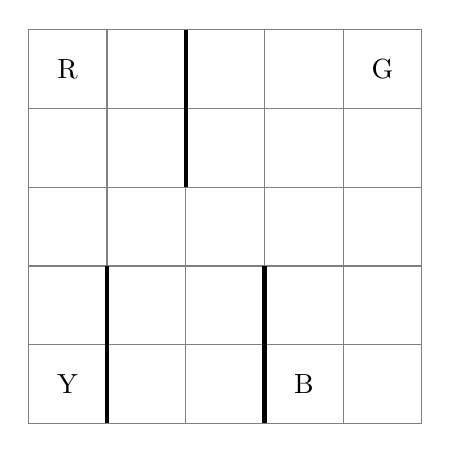
\begin{tikzpicture}
    % Grid
    \draw[step=1,color=gray] (0,0) grid (5,5);
    
    % Walls
    \draw[line width=1.5pt] (2,5) -- (2,3);
    \draw[line width=1.5pt] (1,0) -- (1,2);
    \draw[line width=1.5pt] (3,0) -- (3,2);

    % Pads
    \draw (0.5,4.5) node {R};
    \draw (0.5,0.5) node {Y};
    \draw (3.5,0.5) node {B};
    \draw (4.5,4.5) node {G};
\end{tikzpicture}
\end{document}

    \caption{The Taxi Domain}
    \label{fig:taxi-domain}
\end{figure}

To make the discussion more tangible, let us look at an example, the Taxi
domain, shown in \autoref{fig:taxi-domain}. The agent is a taxi navigating in
this road-map. It must pick up a passenger at one of the 4 pads, A, B, C or D.
Subsequently, it must carry the passenger to a destination, which is also one of
the above four pads. The states of the taxi would then be the location of the
passenger (in one of the four pads, or within the taxi), the destination of the
passenger, and location of the taxi in the map. The actions the taxi can perform
are moving up, down, left or right in the map, as well as pick up a passenger or
drop him at the destination.  Typical options for such a domain would be an
option that can be started anywhere, and has a policy that takes the taxi to the
one of the pads in the shortest possible manner. Such an option is generic, and
does not depend on where the passenger or destination are. The RL agent must
then learn to choose the right option when picking up the passenger.

\begin{figure}[h]
    \center
    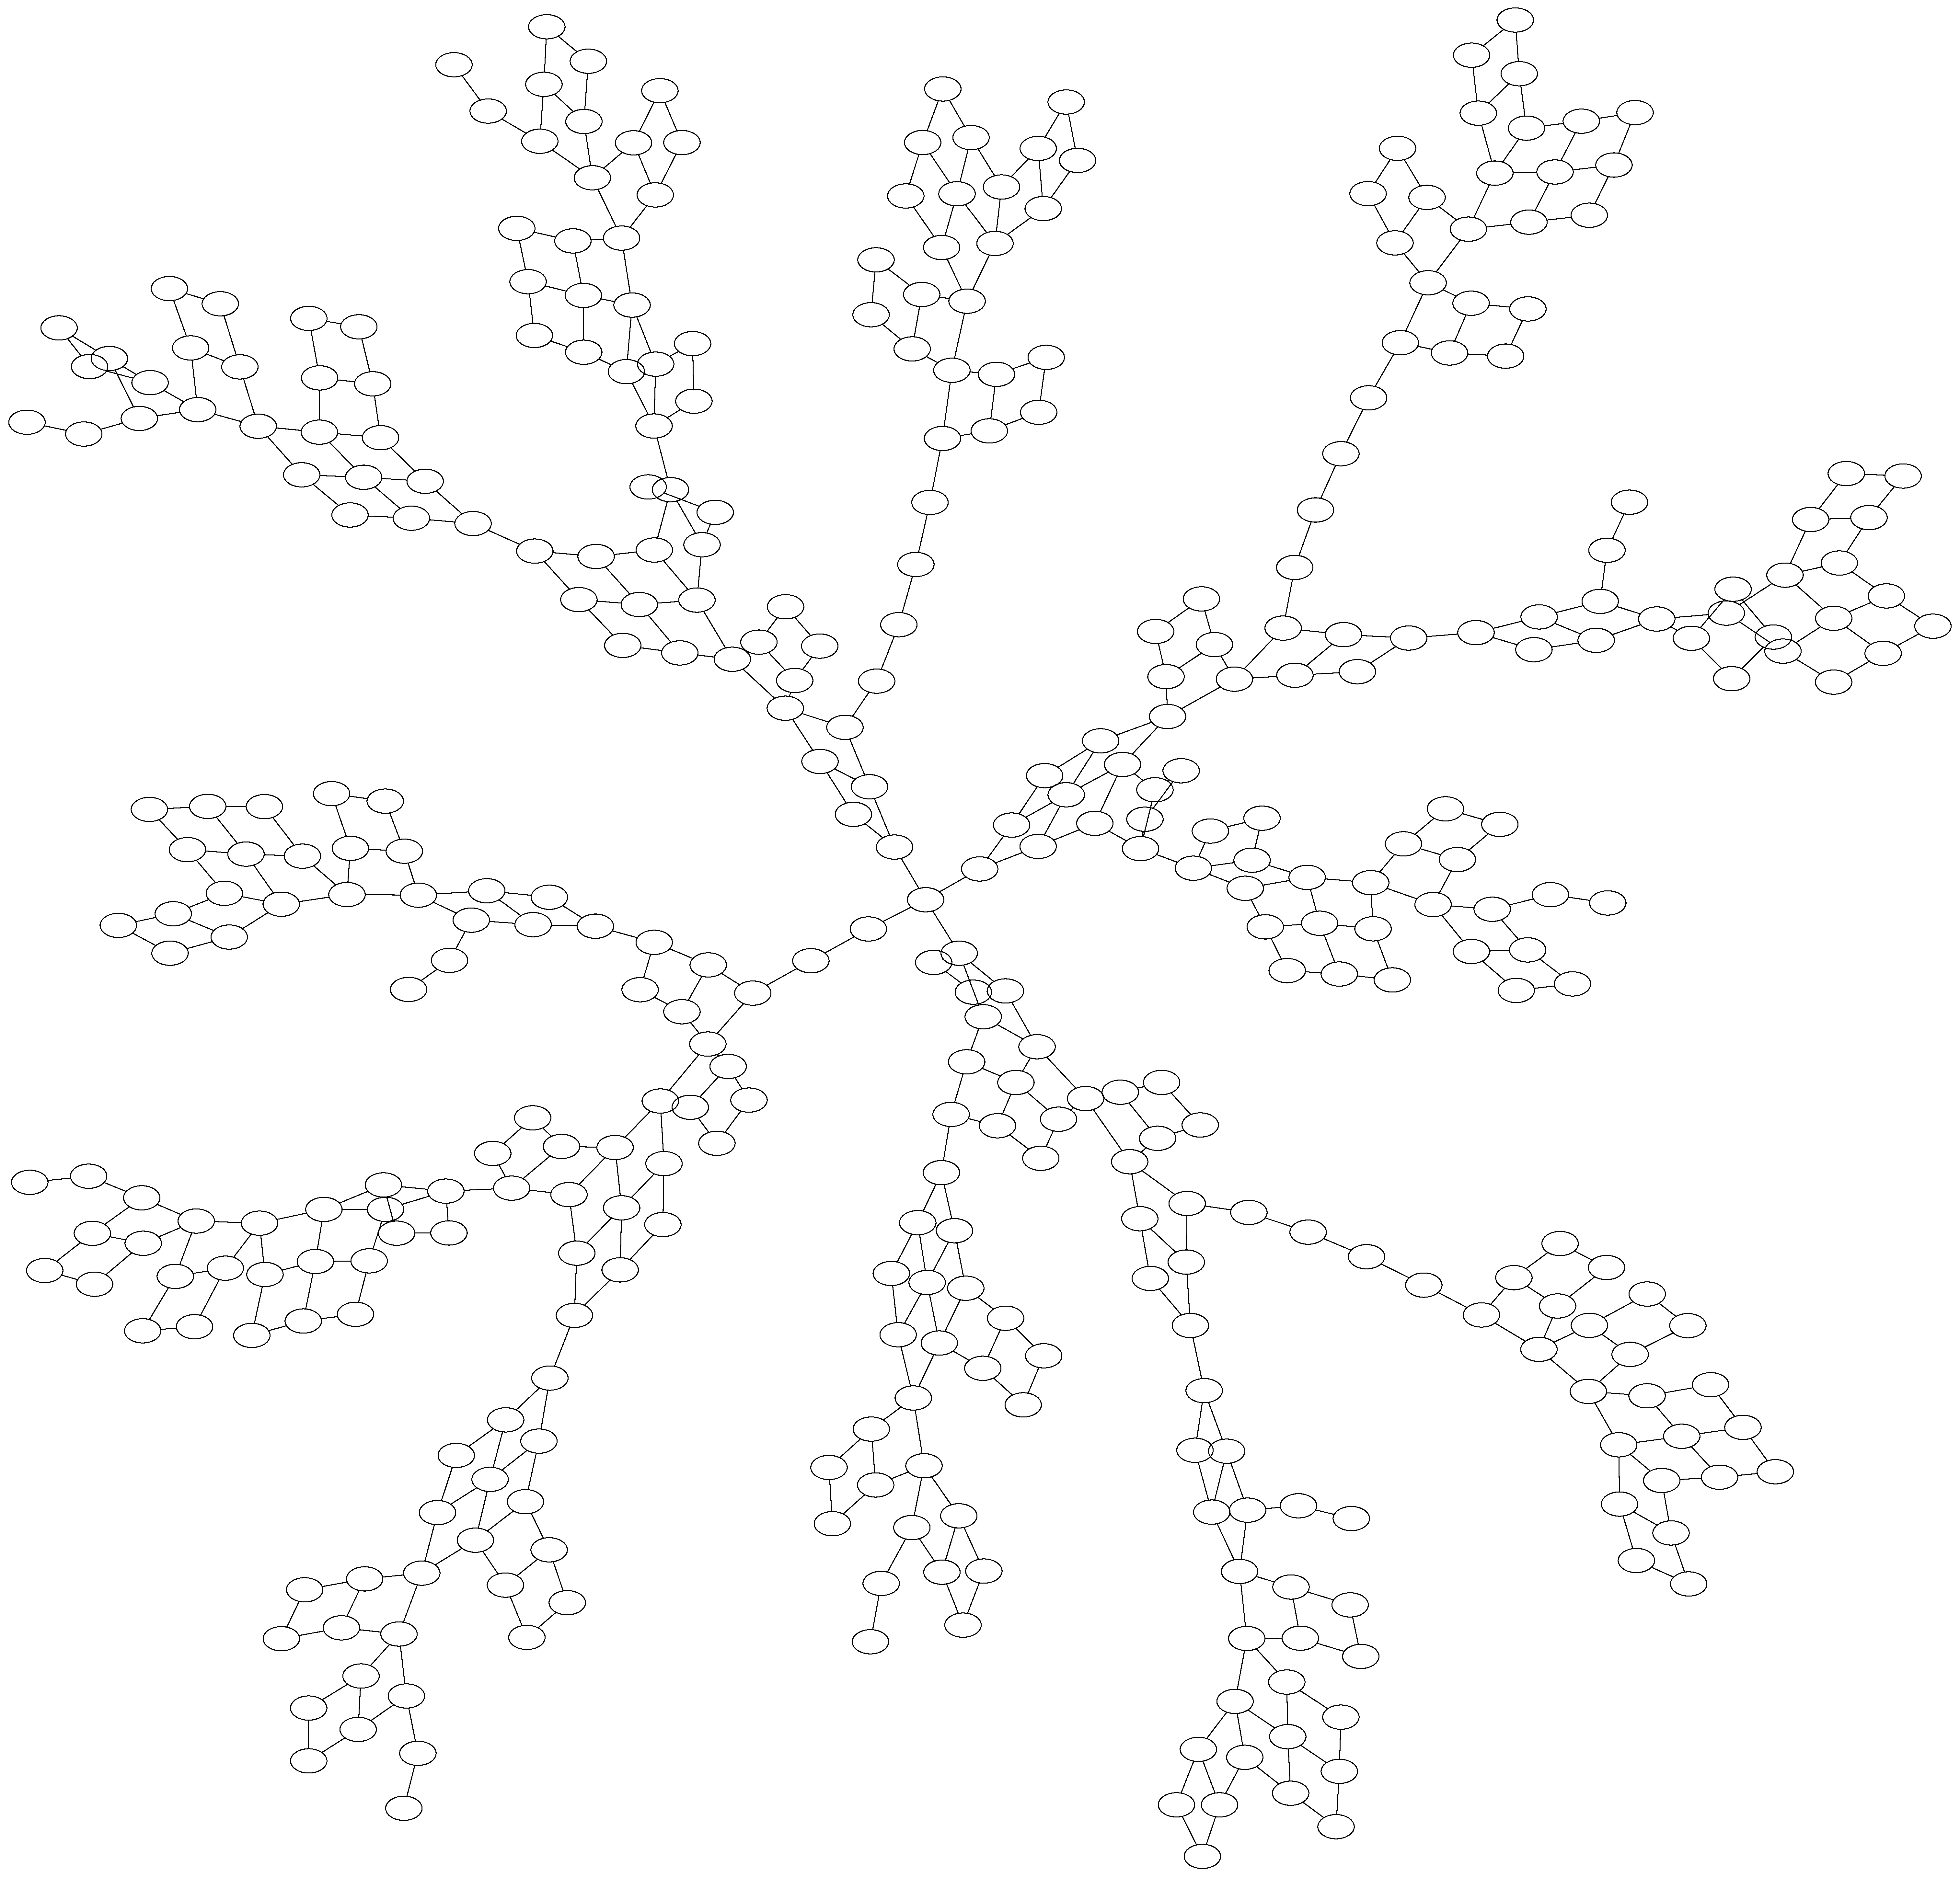
\includegraphics[width=3in]{figures/taxi1}
    \caption{State Space Graph for the Taxi Domain}
    \label{fig:taxi-graph}
\end{figure}

% Graph-based
It is easy to construct a graph $\graph$ out of the state-space described by an
MDP. The states $\states$ become the nodes of the graph, and $\actions$ become
the edges, with the transition probabilites serving as the weights. The edges
are also attributed with the rewards described by $\rewards$. Options can be
viewed to be paths along the graph. The Taxi domain just defined translates to
a graph shown in \autoref{fig:taxi-graph}.

% Constructing Options 
We construct an option `short-circuiting' two states using a policy constructed
from the shortest path on this graph. For every state $x$, we select a state to
be short-circuited $y$ with using a multinomial distribution with weight
proportional to the distance between them in the state space, i.e. $w(x,y)
    \propto d(x,y)^{-r}$. 

Another example of constructing an option on this graph would be to define a
policy that takes any state to a particular one along the shortest path. This is
the approach adopted by Simsek and Barto in \cite{Simsek}, where local maxima of
the betweenness scores are used to identify bottlenecks, and options defined to
reach these bottlenecks optimally from any state.

% Describe Macro-Q and Intra-Option-Q
Several learning algorithms have been proposed for agents using options
\cite{SuttonPrecupSingh1998,BartoMahadevan}. A simple such method is Macro
Q-learning, a generalisation of the Q-learning methods. The MacroQ algorithm
updates the value function only after completion of the option. If the option
$o$ was initiated in the state $s$, and continue for $k$ steps before
terminating in $s'$, the corresponding back-up will be,

\begin{IEEEeqnarray*}{rCl}
    Q(s,o) &=& Q(s,o) + \alpha [ r + \gamma^{k} \max_{o' \in \options_{s'} \cup \actions_{s'}} Q(s',o') - Q(s,o) ].
\end{IEEEeqnarray*}

Another method, Intra-option Q-learning, exploits the experience gathered during
the trajectory, instead of only at the end of it. In this approach, every step
from $s$ to $s'$ using $a \in \actions$ is used to back up the value function of
every option $o \in \options$ which can be used in $s$, and whose policy has a
non-zero probability of using the action $a$ using the following update,

\begin{IEEEeqnarray*}{rCl}
    Q(s,o) &=& Q(s,o) + \alpha [ r + \gamma Q(s',o) - Q(s,o) ].
\end{IEEEeqnarray*}
\noindent
The value-function for every action along the trajectory is also updated, using
the usual Q-learning backups.

% \begin{IEEEeqnarray*}{rCl}
%     x &=& y \\
%       &=& z \\
% \end{IEEEeqnarray*}

% \begin{figure}[s]
%     \centering
%     \includegraphics[width=5in]{filename}
%     \caption{ }
%     \label{fig:high-variance-rtt}
% \end{figure}

%\section{Approach}
\label{sec:approach}

% Explain small world
To answer this question, we look at the analysis of the ``small world
phenomenon'' in social networks by Kleinberg. Kleinberg defines the phenomenon
to be exhibited when when individuals can {\em efficiently} transmit a message
from source to destination knowing only the locations of their immediate
acquaintances with a decentralised algorithm. 
% Statement of Kleinberg's results
Consider a $k$-dimensional lattice of $n$ people \footnote{ Kleinberg's proofs
were limited to the $2$-dimensional case. Martel and Nyugen \cite{Martel2004}
extended them to the $k$-dimensional case }, wherein each person is connected to
one other person outside his/her immediate neighbours, according to the
distribution $P_{r}( u, v ) \propto \dist(u,v)^{-r}$, where $\dist(u,v)$
is the lattice distance between nodes $u$ and $v$, and $r$ is a parameter.
Kleinberg proves (a) that when $r=0$, i.e. the extra connections are uniformly
distributed, any decentralized algorithm will have an expected delivery time
that is exponential in $\tilde{d}$ (the shortest path length between $u$ and
$v$), and (b) when $r=k$, an algorithm can be constructed whose expected
delivery time is only polynomial of small degree in $\tilde{d}$.

Similarly, we define an MDP with options to exhibit the small world property
when an agent can efficiently reach a state of {\em maximal value} using only
its' local information. Using a similarly constructed $k$-dimensional lattice
for $\states$, where two states are connected by primitive actions if they are
neighbours, and by an option with an optimal deterministic policy otherwise. By
relating the distance of two states in the state space, and the difference in
value of the two states, we are able to prove that the expected number of {\em
decisions} an agent will have to make to reach a maximal value state will be poly-logarithmic in
$|\states|$.

\section{Conclusions and Future Work}
\label{sec:conclusions}

% Contributions
% - new scheme for generating options
We have devised a new scheme to generate options based on small world
network model. The options generated satisfy an intuitive criteria, that
the subtasks learnt should be easily composed to solve any other task.
The options also greatly improve the connectivity properties of the
domain.

% - absolutely model-free
Experiments run on standard domains show significantly faster learning
rates using small world options. At the same time, we have shown that
learning small world options can be significantly cheaper than learning
`bottleneck' options. Another advantage of the scheme is that is does
not ever require the model of the MDP. We find it remarkable that we can
learn near optimal behaviour just from the policies of on some tasks


% - theoretical interest
The scheme does not perform any global analysis, and does not require
the model. We have shown that sample-wise, it can be far cheaper than
other bottleneck based methods. Does not lead to state space blow up.
Also is interesting from a theoretical perspective, logarithmic number
of decisions.

% Further work
% - dynamically add/remove options
% - figuring out r
We have as yet not been able to characterise what the exponent $r$
should be in a general domain. Given the ease with which options can be
discovered, it would be interesting to create a dynamic scheme.



\bibliographystyle{alpha}
\bibliography{ewrl}{}

%\newpage
%\appendix

%
\section{Code}
\label{sec:code}
% \lstset{language=TCL, basicstyle=\small, showstringspaces=false, numbers=left, numberstyle=\tiny }
% \lstinputlisting{many2one.tcl}


\end{document}

